\documentclass{beamer}
\usepackage[utf8]{inputenc}
\usepackage[T1]{fontenc}
\usepackage[english]{babel}
\usepackage{amssymb}
\usepackage{soul}
\usepackage{listings}
\usepackage{alltt}
\usepackage{underscore}
\usepackage{verbatim}
\usepackage{graphicx}
\usepackage{ae}
\usepackage{amsmath}
\usepackage{amsfonts}
\PassOptionsToPackage{pdflatex}{graphicx}
\usepackage{algorithm}
\usepackage{algorithmic}
\graphicspath{ {images/} }

\definecolor{listinggray}{gray}{0.9}
\definecolor{lbcolor}{rgb}{0.9,0.9,0.9}


\usefonttheme{professionalfonts}


\title[Degree Project]{Degree Project}
\subtitle{Presentation \#1} 
\author[E. Regla]{Erik Regla} 
\institute[UTalca]{Universidad de Talca}
\date{\today} 

\begin{document}

\begin{frame}
  \titlepage
\end{frame}

\section{Descripción de las pruebas experimentales}

\begin{frame}
  \begin{itemize}
  	\item Advisor: Rodrigo Paredes (rapa)
  	\item Thema: Incremental sorting for arrays with highly redundant classes
  	\item Current Status: A paper, initial tests finished.
  \end{itemize}
\end{frame}


\begin{frame}
    \centering
    \begin{figure}
        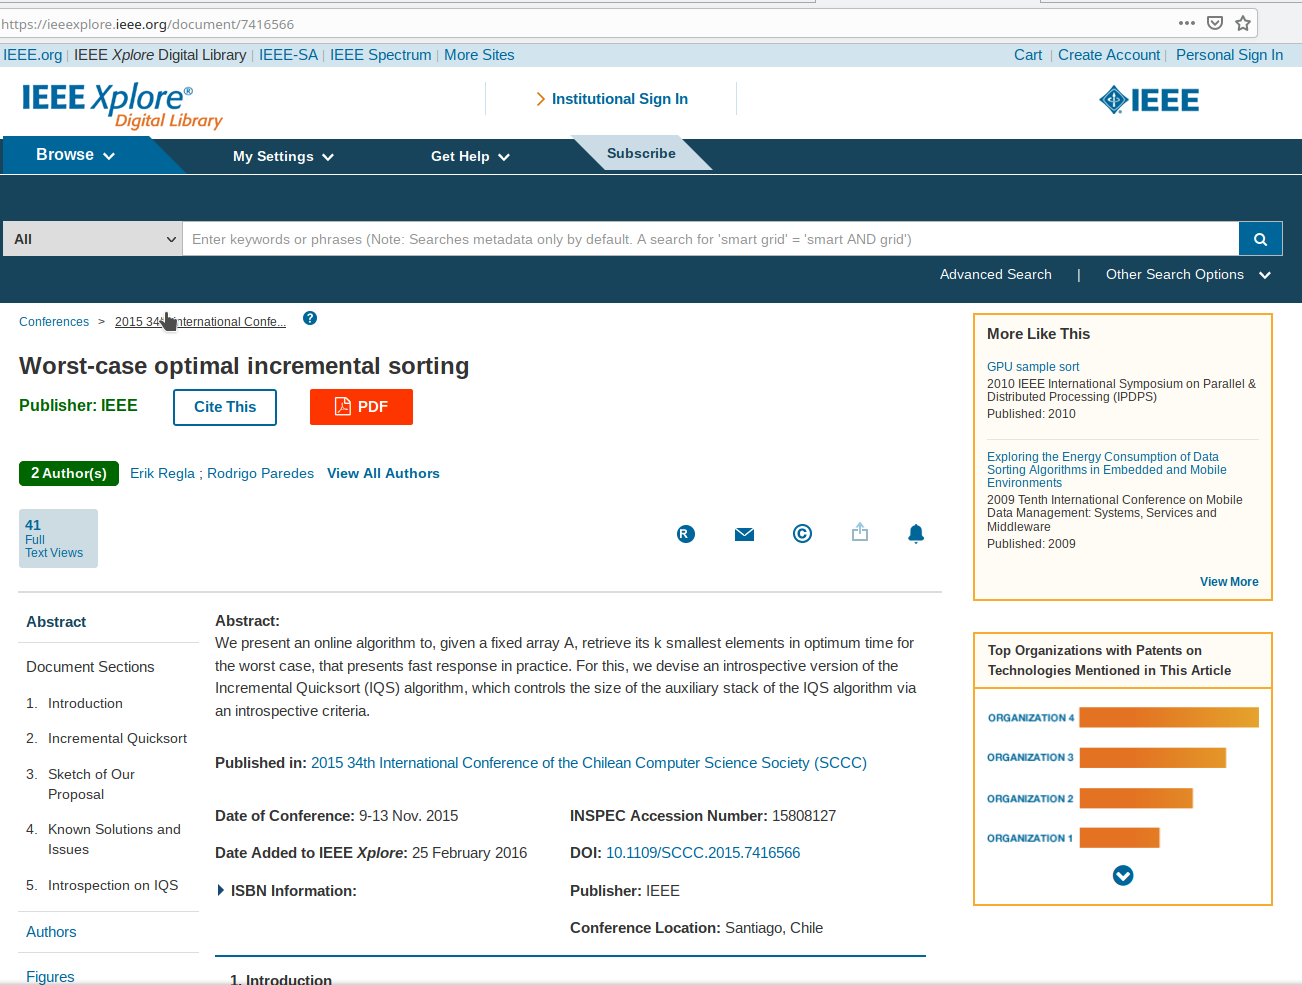
\includegraphics[height=.6\textheight]{paper}\\
        \caption{IIQS implmementation changes the partition method in order to guarantee a partition of linear time and at the same time guarantee a reduction on the search space. (10.1109/SCCC.2015.7416566).}
    \end{figure}
\end{frame}


\begin{frame}
    Current scope is limited as an experimental algorithm design to extend (I)IQS usage for haplotype plot generation, which is an instance of the worst case for IQS but on a discrete space when $C<<n$.\\
\begin{itemize}
    \item Modification 1: Add incremental version of BFPRT algorithm% \pause Success
    \item Modification 2: Change rules for introspective step% \pause Success
    \item Modification 3: Bias the three-way-median returned index% \pause Success
    \item Modification 4: Store the three-way-median result on the stack
\end{itemize}
\end{frame}


\begin{frame}
    \centering
    \begin{figure}
        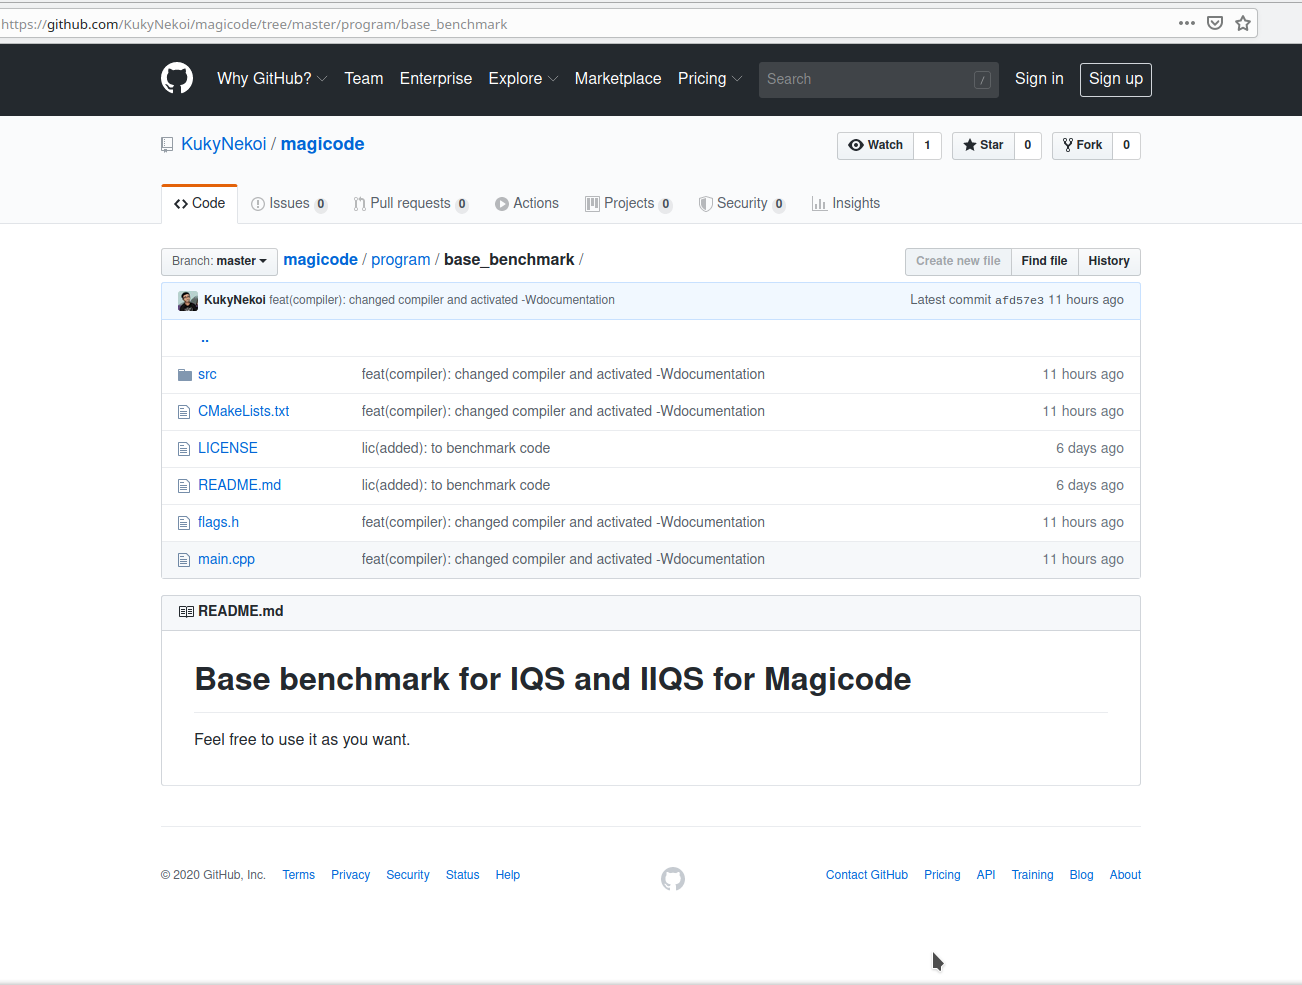
\includegraphics[height=.6\textheight]{repo}\\
        \caption{Implementation for the tests available under GNU GPL license at \href{https://github.com/KukyNekoi/magicode/tree/master/program/base_benchmark}{GitHub}}
    \end{figure}
\end{frame}


\begin{frame}
\begin{itemize}
    \item Scope: Experimental design, setup and experimentation
    \item Part of magicode, a personal research on FPGA implementation of hardware accelerators for similarity search (the original thema).
    \item Got someone interested on using this algorithm for solving haplotype plots
\end{itemize}
\end{frame}
  
\begin{frame}
\centering
		FIN
\end{frame}



\end{document}
